\documentclass[a4paper]{report}
\usepackage{bookmark}
\usepackage[utf8]{inputenc}
\usepackage{authblk}
\usepackage{amsmath,amsfonts,amsthm,amssymb,mathtools}
\usepackage[english]{babel}


%% theorem, lemma, proof, etc. %%
%% for unnumbed use \newtheorem* and delete section in [---] %%
\newtheorem{theorem}{Theorem}[section]
\newtheorem{corollary}{Corollary}[theorem]
\newtheorem{lemma}[theorem]{Lemma}
\newtheorem{proposition}[theorem]{Proposition}

\theoremstyle{remark}
\newtheorem{remark}{Remark}
\newtheorem{example}{Example}[chapter]

%% \thetheorem %%

\usepackage{enumitem}
\usepackage{graphicx}
\graphicspath{ {./images/} }
\usepackage{subcaption}
\usepackage{tikz}
\usetikzlibrary{decorations.fractals}
\usepackage{float}
\usepackage{dsfont}
\usepackage{geometry}
\geometry{
    a4paper,
    left=30mm,
    right=30mm,
    top=20mm,
    bottom=20mm,
}

%%%% hyperref %%%%
\usepackage{url}
\usepackage{hyperref} % for link
\hypersetup{
    colorlinks=true,
    allcolors=black,
}
\usepackage{cleveref}
%%% fancyhdr %%%% for footer and Hader of document
\usepackage{fancyhdr}
%\pagestyle{fancy}
%\lhead{lest hand head} %% left Hader %%
%\rhead{Measure Theory} %% right Hader %%
\cfoot{\thepage} %% central footer %%

\setlength{\headheight}{14.49998pt}

%% for code 
\usepackage{xcolor}
\usepackage{tcolorbox}
\usepackage{listings}
\lstset{language=Python,
        basicstyle=\ttfamily\small,
        %% keywordstyle=\color{blue},
        commentstyle=\color{black},
        %% stringstyle=\color{orange},
        showstringspaces=false,
        breaklines=true,
        frame=single,
        %% numbers=left,
        %% numberstyle=\tiny\color{gray}
}

%%% spacing in document %%%
\usepackage{setspace}
\onehalfspacing

\title{MCMC}
\author{Azmain Biswas}
\date{April 2023}

\begin{document}

 \newcommand{\cosec}{\operatorname{cosec}}
\newcommand{\tx}[1]{\text{#1}}
\newcommand\numberthis{\addtocounter{equation}{1}\tag{\theequation}}   

\begin{titlepage}
    \begin{center}

        \vspace{0.5cm}

        \Large{\textbf{A M.Sc Thesis\\ on}}\\
        \huge{\textbf{Simulation and \\ Markov Chain Monte Carlo}}

        \vspace{0.5cm}
        \large{\textbf{by}}\\ 
        \Large{\textbf{Azmain Biswas}}\\ 
        \Large{\textbf{Enrollment No.: 2022MAM008}}\\ 
        \Large{under the supervision of}\\ 
        \Large{\textbf{Prof. M. Mitra}}

        \vspace{0.5cm}

        
\includegraphics[scale = 0.1]{images/IIEST_Shibpur_Logo.svg.png}

        \vspace{0.5cm}

        \Large{{
                INDIAN INSTITUTE OF ENGINEERING SCIENCE AND TECHNOLOGY, Shibpur\\ 
                \textbf{Department of Mathematics}
        }}\\
        \vspace*{0.5cm}
        \large{{Submitted for the partial fulfillment of the requirements for the award of the degree of}}\\
        \Large{\textbf{M.Sc. in Applied Mathematics}}
    \end{center}
\end{titlepage}

\vspace{10cm}
\begin{center}
    \LARGE{\textbf{CERTIFICATE}}
\end{center}
\large
\vspace*{2cm}
This is to certify that the Term Paper on \textbf{"Simulation and Markov Chains Monte Carlo"} submitted by Azmain Biswas to the Department of Mathematics, Indian Institute of Engineering Science and Technology, Shibpur, Howrah-711103, for 3rd semester of Master of Science in Applied Mathematics is a record of project work carried out by him under my supervision. \\
The result of this project work or any part thereof has not been submitted for any degree or diploma.
\vspace{4cm}
\begin{flushright}
    Prof. M. Mitra\\
    Department of Mathematics\\
    Indian Institute of Engineering Science and Technology\\
    Shibpur, Howrah.
\end{flushright}

\vspace{5cm}

\begin{center}
    \LARGE{\textbf{Acknowledgment}}
\end{center}
\vspace{2cm}
    At outset, I would like to express my thanks to my supervisor, Prof. M. Mitra, for a very interesting project. It has been a great pleasure to work under his guidance and I have learned a lot from his way of thinking and his approach to a problem. 
    \vspace{0.2cm}

    I am also indebted to Prof. Pritha Das, Head of the Department of Mathematics, Indian Institute of Engineering Science and Technology, Shibpur, for allowing me to utilize the infrastructure of the department. 

    \vspace{0.2cm}
    At various stages, I received encouragement and inspiration from most of the faculty members of the department. I would like to thank them all for their invaluable words of advice.

    \vspace{0.2cm}
    I have benefited greatly from the advantages of the \TeX-group software typing systems, the use of which has contributed much to simplify the typing of long mathematical expressions involved in my work.

    \vspace{0.2cm}
    Additionally, I would like to thank the Python Software Foundation for their software, without which I could not have completed this project.

    \vspace{0.2cm}
    I would like to thank my parents and friends for being so supportive of my career and life choices, as well as for making me happy.

    \vspace{2cm}
    \begin{flushright}
        Azmain Biswas
    \end{flushright}

\tableofcontents
\listoffigures
\chapter{Introduction}

In the ever-evolving landscape of mathematical and statistical research and application, 
the integration of simulation techniques has emerged as a powerful tool to unravel complex phenomena, validate theoretical frameworks, 
and facilitate a deeper understanding of intricate mathematical structures. 
Simulation is a computer-based exploratory exercise that aids in understanding how
the behavior of a random or even a deterministic process changes in response to
changes in input or the environment. It is essentially the only option left when exact
mathematical calculations are impossible, or require an amount of effort that the user
is not willing to invest. Even when the mathematical calculations are quite doable, a
preliminary simulation can be very helpful in guiding the researcher to theorems that
were not a priori obvious or conjectured, and also to identify the more productive
corners of a particular problem. Although simulation in itself is a machine-based
exercise, credible simulation must be based on appropriate theory. A simulation
algorithm must be theoretically justified before we use it.

The classic theory of simulation includes such time-tested methods as the original Monte Carlo, 
Inverse Transform method, Accept-Reject method, Bivariate techniques  
from standard distributions in common use. They involve a varied degree of sophistication. 
Markov chain Monte Carlo is the name for a collection of simulation algorithms for simulating from
the distribution of very general types of random variables taking values in quite
general spaces. MCMC methods have truly revolutionized simulation because of an
inherent simplicity in applying them, the generality of their scopes, and the diversity
of applied problems in which some suitable form of MCMC has helped in making
useful practical advances. MCMC methods are the most useful when conventional
Monte Carlo is difficult or impossible to use.

Simulation depend on various theoretical aspect such as 
The weak law of Large Number, The Central limit theory, The sample mean and sample variance etcetera.

There are various type of simulation technique in standard simulation theory 
such as,

\begin{enumerate}
	\itemsep=-.3em
	\item The Inverse Transform Method
	\item Accept-Reject Algorithm
	\item Bivariate Techniques
	\item Ordinary Monte Carlo
	\item Importance Sampling
	\item Markov Chain Monte Carlo
\end{enumerate}

This project work focus mainly on these simulation techniques.

In Chapter 2, we discuss about how to generate random variable both
uniform and continuous, by using method like The Inverse Transform Method, 
Accept-Reject Algorithm, Bivariate Techniques.

In Chapter 3, we focus on Ordinary Monte Carlo and how to use it to solve problem like evaluating integration and evaluating the value of $\pi$.

In Chapter 4, the focus shifts to Importance Sampling and how it beneficial
from Ordinary Monte Carlo by some example. Learn about how to chose 
optimal Importance sample distribution.

\section{Mathematical Preliminaries}

\begin{definition}[Probability Space]
	A probability spacs is a triple $(\Omega, \mathcal{F}, P)$ consisting of:
	\begin{enumerate}
		\item[(a)] the sample space $\Omega$ (an arbitrary non-empty set)
		\item[(b)] a non-empty collection of subsets $\mathcal{F} $ of $ \Omega $,
		      called \textit{sigma field} of subspace of $ \Omega $, 
		      such taht,
		      \begin{itemize}
			      \item[(i)] $ \Omega \in \mathcal{F} $
			      \item[(ii)] if $ A \in \mathcal{F} $, then $ A^{c}\in \mathcal{F}  $
			      \item [(iii)] if $ A_n\in \mathcal{F},\ n=1,2,\ldots $, then $ \cup_n=1^{\infty}A_n \in \mathcal{F}  $
		      \end{itemize}
		\item [(c)] a probability measure $ p:\mathcal{F}\to [0,1] $, which is a real valued function on $ \mathcal{F} $
		      such that,
		      \begin{itemize}
			      \item [(i)] $ P(A) \ge 0 $ for all $ A\in \mathcal{F} $
			      \item [(ii)] $ P(\Omega) = 1 $
			      \item [(iii)] if $ A_1,A_2,\ldots $ are disjoint sets in $ \mathcal{F} $, then $ P(\cup_n A_n) = \sum_{n} P(A_n)  $.
		      \end{itemize}
	\end{enumerate}
\end{definition}

\begin{definition}[Conditional Probability]
	Let $A$, $B$ be general events with respect to some sample space $ \Omega $,
	and suppose $ P(A)>0 $. The \textit{conditional probability} of $ B $ given $ A $ is defined as 
	\[
		P(B|A) = \frac{P(A\cap B}{P(A)}.
	\]
\end{definition}

\begin{theorem}[Bayes's Theorem]
	Let, $ \{ A_1,A_2,\ldots,A_n \} $ be a partition of sample space $ \Omega $. 
	Let $ B $ be a some fixed event. Then
	\[
		P(A_j|B) = \frac{P(B|A_j)P(A_j)}{\sum_{i=1}^{n}P(B|A_i)P(A_i) }.
	\]
\end{theorem}

\begin{definition}[Random Variable]
	Let, $ \Omega $ be a sample space corresponding to some experiment and let 
	$ X:\Omega\to \mathds{R} $ be a function from the sample space to the real line. 
	Then $ X $ is called a \textit{random Variable}
\end{definition}

\begin{definition}[Cumulative Distribution Function]
	The cumulative distribution function(CDF) or simply distributed function, $ F $ of 
	a random variable $ X $ is define for any real number $ x $ by
	\[
		F(x) = P(X \le x).
	\]
\end{definition}

\begin{definition}[Probability Mass Function]
	For a discrete random variable $ X $ we define its Probability mass function(pmf)
	$ p(x) $ by
	\[
		p(x) = P(X=x)
	\]
	and we have,
	\[
		\sum_{i\in \Lambda} p(x_i) = 1. \text{ and } p_i \ge 0. 
	\]
\end{definition}

\begin{definition}[ Probability Density Function ]
	For a continuous random variable if there is a non-negative function $ f(x) $
	defined for all real number $ x $ and having the property that for any set $ C\subset \mathds{R} $,
	\[
		P(X\in C) = \int_{C}f(x) dx 
		.\]
	The function $ f $ is called probability density function(pdf) of the random variable $ X $.
\end{definition}

The relation between CDF and pdf is express by,
\[
	F(a) = P(X\in (-\infty, a]) = \int_{-\infty}^{a} f(x) dx.
\]

\begin{definition}[Exception]
	If $ X $ is a random variable,
	then the \textit{exception} or \textit{expected value} of $ X $, also called the mean of $ X $ and denoted by $ E(X) $, is define by
	\[
		E(X) = \int xdF(x) 
	\]
\end{definition}

\begin{definition}[Variance]
	If $ X $ is a random variable with mean $ E(X) $, then the variance of $ X $,
	denoted by $ Var(X) $, is define by,
	\[
		Var(X)=E\left( (X-E(X))^{2} \right)
	\]
\end{definition}

\begin{theorem}[The Weak Law of Large Numbers]
	Let $X_1,X_2,\ldots$ be a sequence of in dependent and identically distributed 
	random variables having mean $ \mu $, Then, for any $ \epsilon >0 $,
	\[
		P \left( \left|\frac{X_1+X_2+ \ldots + X_n }{n} - \mu \right| > \epsilon \right) \to 0 
	\]
\end{theorem}

\begin{theorem}[The Central Limit Theorem]
	Suppose $X_1, X_2, \ldots  $ is a sequence of i.i.d random variables with 
    $E[X_i]=\mu$ and $\text{Var}[X_i]=\sigma ^{2} < \infty$. Then, 
	\[
		\lim_{n \to \infty} P\left( \frac{X_1+\ldots+X_n - n\mu}{\sigma \sqrt{n } } < n \right) = \Phi(Z)
	\]
	Were, $\Phi(Z)$ denote the distribution function of a standard normal distribution.
\end{theorem}

\subsection*{Sample Mean and Sample Variance}
Suppose that $ X_1,X_2,\ldots,X_n $ are independent random variable having the same
distribution function. Let $ \mu $ and $ \sigma ^{2} $ denote, respectively 
their mean and variance that is, $ \mu = E(X_i) $ and $ \sigma ^{2} = Var(X_i) $.
The quantity
\[
	\bar{X} \equiv \sum_{i=1}^{n} \frac{X_i}{n}
\]

which is the arithmetic average of the $ n $ data values, is called the \textit{sample mean}.
When the population mean $ \mu $ is unknown, the sample mean is often used to estimate $ \mu .$

Because, 
\begin{align*}
	E(\bar{X}) & = E\left( \sum_{i=1}^{n} \frac{X_i}{n} \right) \\ 
	           & = \sum_{i=1}^{n} \frac{E(X_i)}{n}              \\ 
	           & = \frac{n \mu}{n} = \mu
\end{align*}

if follows that $ \bar{X} $ is an unbiased estimator of $ \mu $, where we say that an estimator
of parameter is an unbiased estimator of that an estimator of a parameter is an unbiased estimator
of that parameter if its expected value is equal to the parameter.

The quantity $ S ^{2} $, define by 
\[
	S ^{2} = \frac{\sum_{i=1}^{n}(X_i - \bar(X))^{2} }{n-1}
\]
is called the \textit{sample variance} .

Whish is also unbised of $ \sigma ^{2} $

\chapter{Generating Random Variables}

\section{Generating Discrete Random Variables}

Main component of a simulation study is the ability to generate random number, where a random number represents the value of random variable uniform
distribution on $(0,1)$.
\subsection{Pseudorandom Number Generation}
Random numbers were originally either manually or mechanically generated, by using spinning wheels or dice rolling or card shuffling
but the modern approach is to use a computer to successively generate pseudorandom numbers.

One of the common approaches to generate pseudorandom numbers starts with an initial value $x_0$, called seed, and then recursively computes
successive values $x_n, n\ge1$, by letting
\begin{equation}
	\label{MCM}
	x_n = a x_{n-1} \text{ modulo } m
\end{equation}
where $a$ and $m$ are given positive integers, and where the equation (\ref{MCM}) means that $ax_{n-1}$ is divided by  $m$ and remainder is taken as the
value of $x_n$. Thus, each value of $x_n$ is either $0,1, \ldots, m-1$ and the quantity $x_n / m$ is Pseudorandom number and follows
an approximation to the value of a uniform $(0,1)$ random variable.

The approach specified by equation (\ref{MCM}) to generate random numbers is called the Multiplicative Congruential Method.

Another method is
\[
	x_n = (a x_{n-1}+c) \text{ modulo } m
\]
this method is known as \textit{Mixed Congruential Generators} or \textit{Linear congruential Generations (LCGs)} where $c$ is a non-negative integer.

\subsection{The Inverse Transform Method}
Suppose we want to generate the value of a discrete random variable $X$ having probability mass function
\[
	P(X=x_i)=p_i, \ i = 0,1, \ldots , \ \sum_ip_i =1
\]
To do this, we generate a random number from a uniform distribution $(0,1)$ $U$, and set
\[
	X=
	\begin{cases}
		x_0 \text{ if } U<p_0                                         \\
		x_1 \text{ if } p_0\le U\le p_0+p_1                           \\
		\vdots                                                        \\
		x_j \text{ if } \sum_{i=0}^{j-1}p_i\le U\le \sum_{i=0}^{j}p_i \\
		\vdots
	\end{cases}
\]
Since, for $0<a<b<1, P(a\le U<b) = b-a$, we have,
\[
	P(X=x_j)=P\left( \sum_{i=0}^{j-1}p_i\le U< \sum_{i=0}^{j}p_i \right) = p_j
	.\]
So, $X$ has the desired distribution.

\begin{example}[Bernoulli Distribution]
	Let, $X\sim Ber(p)$ where p is success probability  i.e.  $P(X=0)= 1-p$ and  $P(X=1)=p$ and $0\le p \le 1$.
	Then, to generate $X$ we first generate $U \sim U[0,1]$ then, we set

	\[
		X=
		\begin{cases}
			1, \text{ if } U\le p \\
			0, \text{ if } U> p
		\end{cases}
	\]
	Hence, $X$ follows Bernoulli Distribution with the parameter $p$.\\
	\textbf{Algorithm for Inverse Transform Algorithm for Generating Bernoulli Distribution:}\\
	STEP 1: Generate a random variable $U\sim U[0,1]$.\\
	STEP 2: If $U\le p$ set $X=1$ or set  $X=0$. \\
	STEP 3: Go to  STEP 1.

	\begin{figure}[H]
		\centering
		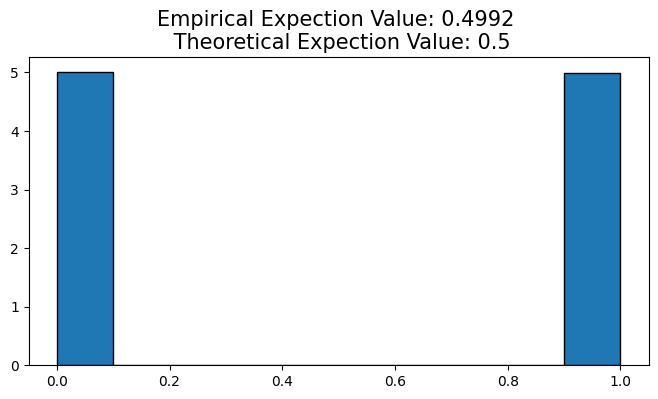
\includegraphics[width=0.6\textwidth]{ber_ITA.png}
		\caption{Inverse Transform method for generating  Bernoulli random numbers with $p=0.5$}
	\end{figure}
\end{example}

\begin{example}[Binomial Distribution]
	Let, $X\sim Bin(n,p)$ then,  $X$ has probability mass function
	\[
		f(r) = P(X=r) = {n\choose r}p^{r}(1-p)^{n-r},\  i = 1,2, \ldots
	\]
	The generation of $X\sim Bin(n,p)$ by Inverse Transform Algorithm can be tedious. We can use the relation between Binomial and Bernoulli distribution.
	If $x_i \sim Ber(p), \forall i = 1,2, \ldots, n$ then, $\sum_{i=1}^{n} x_i\sim Bin(n,p)$.

	Hence, by generating $x_i$ $n$ independent random variable from Bernoulli distribution and summing them we get binomial distribution
	\begin{figure}[H]
		\centering
		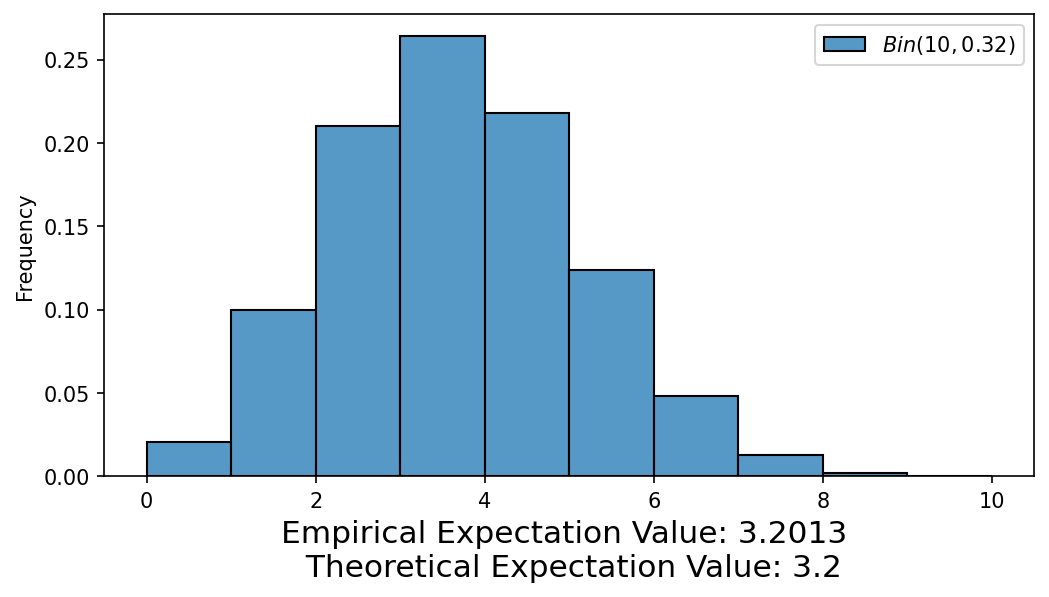
\includegraphics[width=0.6\textwidth]{images/bin_ITA.png}
		\caption{Generating  binomial random numbers with $n=10$ and  $p=0.32$}
	\end{figure}
\end{example}

\section{Generating Continuous Random Variables}

\subsection{The Inverse Transform Algorithm}
To generate Continuous random variables The Inverse Transform Algorithm is very important method. It is based on a following theorem.
\begin{theorem}
	\label{ITA theorem}
	Let $U$ be a uniform  $(0,1)$ random variable. For any continuous distribution function  $F$ the random variable  $X$ defined by
	\[
		X=F^{-1}(U)
	\]
	has distribution $F$.
\end{theorem}
\begin{proof}
	Let, $F_X$ denote the distribution function of  $X=F^{-1}(U)$. Then,
	\begin{align*}
		F_X(x) & = P(X\le x)         \\
		       & = P(F^{-1}(U)\le x) \\
	\end{align*}
	Since, $F$ is a cumulative distribution function it follows that $F(x)$ is monotonic increasing function of  $x$ and range of  $F(x)$ is  $(0,1)$.
	Then,
	\begin{align*}
		F_X(x) & = P\left(F\left(F^{-1}(U)\right)\le F(x)\right) \\
		       & = P(U\le F(x))                                  \\
		       & = F(x) \text{ since $U\sim U(0,1)$ }
	\end{align*}
\end{proof}

The above theory tells us we can generate a random variable $X$ from the continuous distribution function  $F$ by generating a random number $U\sim U(0,1)$
and setting $X=F^{-1}(U)$.

\begin{example}[Exponentian Distribution]
	\label{exponential distribution}
	Suppose we want to generate a random variable $x\sim Exp(\lambda)$, then its probability density function is
	\[
		f(x) = \lambda e^{-\lambda x}.
	\]
	Hence, The cumulative distribution function is,
	\[
		F(x) = 1-e^{\lambda x}
	\]
	if we let $x=F^{-1}(u)$, then,
	\begin{align*}
		u   & =F(x)=1-e^{-\lambda x}       \\
		1-u & = e ^{-\lambda x}            \\
		x   & = - \frac{\ln(1-u)}{\lambda}
	\end{align*}

	Hence, we can generate an exponential random variable with parameter 1 by generating a uniform $(0,1)$ random number $U$ and then setting
	\[
		X = F^{-1}(U) = -\frac{\ln(1-U)}{\lambda}.
	\]
	We see that if $U\sim U(0,1)$ then also $1-U\sim U(0,1)$ thus  $\ln(1-U)$ has the same distribution as  $\ln(U)$ so,
	\[
		X = F^{-1}(U) = -\frac{\ln(U)}{\lambda}.
	\]
	will also work. If we use second expression then the algorithm will take less computing power hence less time.
	\begin{figure}[H]

		\centering
		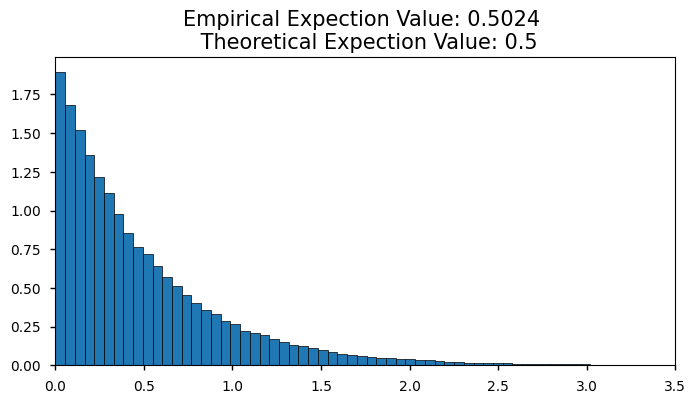
\includegraphics[width=0.6\textwidth]{images/exp_ITA.png}
		\caption{Inverse Transform method for generating $Exp(2)$}
	\end{figure}
\end{example}
\begin{example}[Gamma Distribution]
	Let $X\sim G(n,\lambda)$ Then, its probability  mass function is given by,
	\[
		f(x) = \frac{1}{\Gamma(n)}\lambda^{n}x^{n-1}e^{-\lambda x}
	\]

	We know if $X_i\sim Exp(\lambda) \forall i = 1,2, \ldots ,n$ then  $Y=\sum_i X_i \sim G(n,\lambda)$. As,

	\begin{align*}
		M_{Y}(t) = E \left[ e^{tY} \right] = E\left[ e^{\sum_{i=1}^{n} X_it  }\right] & = E\left[ \prod_{i=1}^{n} e^{X_it} \right]                                                \\
		                                                                              & =\prod_{i=1}^{n} E\left[  e^{X_it} \right] \text{ As all $X_i$ are independent }          \\
		                                                                              & = \prod_{i=1}^{n}\frac{\lambda}{\lambda-t} = \left( \frac{\lambda}{\lambda-t} \right)^{n}
	\end{align*}

	Then, Generating  $n$ number of $X_i\sim Exp(\lambda)$
	and summing them we can easily generate a random variable which follows gamma distribution
	\begin{figure}[H]

		\centering
		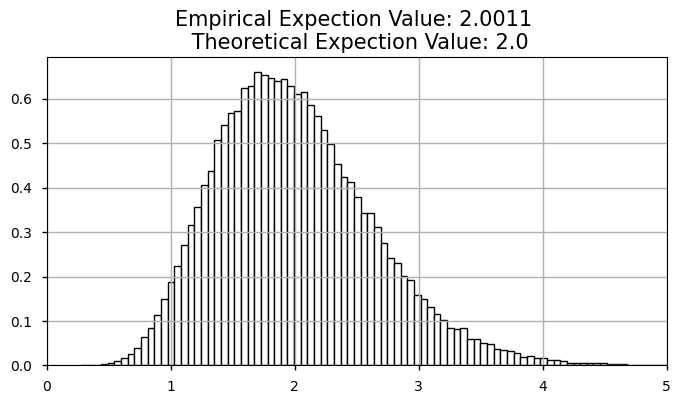
\includegraphics[width=0.6\textwidth]{images/gamma_ITA.png}
		\caption{$G(10,5)$ generated by summing of $Exp(5)$}
	\end{figure}
\end{example}

\subsection{Accept - Reject Method}
The accept–reject method is useful when it is difficult to directly simulate $f(x)$ but we can generate another density $g(x)$ such that $f(x)/g(x)$
is uniformly bounded and it is much easier to simulate $g(x)$. We simulate  $X$ from  $g$, and retain it or toss it according
to a probability proportional to $f(x)/g(x)$.
Because an $X$ value is either retained
or discarded, depending on whether it passes the admission rule, the method is called
the accept–reject method. The density $g(x)$ is called the envelope density.

The method proceeds as follows, \\
STEP 1: Find a density $g$ and a finite constant  $c$ such that  $\frac{f(x)}{g(x)}\le c \ \forall x$.\\
STEP 2: Generate $X\sim g$.\\
STEP 3: Generate  $U\sim U(0,1)$, independent of  $X$. \\
STEP 4: Retain this generated value  $X$ if  $U\le \frac{f(x)}{cg(x)}$.\\
STEP 5: Repeat the same until the required number of $n$ values of  $X$ has been obtained.\\

The following theorem supports the method.
\begin{theorem}
	Let $X\sim g$, and  $U$, independent of, be a distributed as $U[0,1]$. Then the conditional density of $X$ given that
	$U\le \frac{f(X)}{cg(X)}$ is $f$.
\end{theorem}
\begin{proof}
	Denote the CDF of $f$ by $F$. Then,
	\begin{align*}
		P\left( X\le x|U\le \frac{f(X)}{cg(X)} \right) & = \frac{P\left( X\le x, U\le \frac{f(X)}{cg(X)} \right)}{P\left( U\le \frac{f(x)}{cg(x)} \right)}                            \\
		                                               & = \frac{\int_{-\infty}^{x}\int_{0}^{\frac{f(t)}{cg(t)}}g(t)dudt}{\int_{-\infty}^{\infty}\int_0^{\frac{f(t)}{cg(t)}}g(t)dudt} \\
		                                               & = \frac{\int_{-\infty}^{x}f(t)dt}{\int_{-\infty}^{\infty}f(t)dt} = \frac{F(x)}{1}= F(x).
	\end{align*}
\end{proof}

\begin{example}[Generating a Normal Random Variable]
	\label{generate normal}
	To generate a standard normal variable $Z$ i.e. $Z\sim N(0,1)$, note first that the absolute value of  $Z$ has probability density function
	\begin{equation}
		\label{abs std normal}
		f(x) = \frac{2}{\sqrt{2\pi}}e^{- \frac{x^{2}}{2}} \ 0\le x \le \infty.
	\end{equation}
	Then, we can choose $g$ as the exponential density function with mean 1 i.e.
	\[
		g(x) = e^{-x}\ 0\le x\le \infty
	\]
	Now,
	\[
		\frac{f(x)}{g(x)} = \sqrt{\frac{2}{\pi}} e^{x-\frac{x^{2}}{2}}
	\]
	and so the maximum value of $f(x)/g(x)$ occurs at the value of $x$ that maximize $x-x^2 /2$ hence $x=1$ so we take
	\[
		c = \max_x \frac{f(x)}{g(x)} = \frac{f(1)}{g(1)} = \sqrt{\frac{2e}{\pi}}.
	\]
	Now,
	\[
		\frac{f(x)}{cg(x)} = \exp\left( x-\frac{x^2}{2}-\frac{1}{2} \right) = \exp\left( \frac{-(x-1)^2}{2} \right)
	\]
	Then, its follows that we can generate the absolute value of a standard normal random variable as follows: \\
	STEP 1: Generate $X\sim Exp(1)$. \\
	STEP 2: Generate $U\sim U(0,1)$, independent of $X$.\\
	STEP 3: If  $U\le \exp\left( -(X-1)^2 /2 \right)$, retain  $X$, Otherwise, return to Step 1.\\

	Once, we have simulated a random variable $X$ having density function as in
	Equation (\ref{abs std normal}) we can obtain a standard normal $Z$ by letting
	$Z$ be equally likely to be either  $X$ or  $-X$.
	In Step 3, the value $X$ is accepted if  $U\le \exp\left( -(X-1)^2 /2 \right)$, which is equivalent to $- \ln U\ge (X-1)^2 /2$.
	However, in Example (\ref{exponential distribution}) we have seen that $-\ln{U}\sim Exp(1)$ When $U\sim U(0,1)$.

	So, summing up, we can generate the standard normal random variable $Z$ as follows:\\
	STEP 1: Generate independent $X_1, X_2\sim Exp(1) $\\
	STEP 2: If $X_2\ge (X_1-1)^2 /2$ retain $X_1$. Otherwise, return to Step 1.\\
	STEP 3: Generate $U\sim U(0,1)$ and set,
	\begin{eqnarray*}
		Z=
		\begin{cases}
			X_1 \text{ if } U\le \frac{1}{2}, \\
			X_1 \text{ if } U> \frac{1}{2}.
		\end{cases}
	\end{eqnarray*}

	\begin{figure}[H]

		\centering
		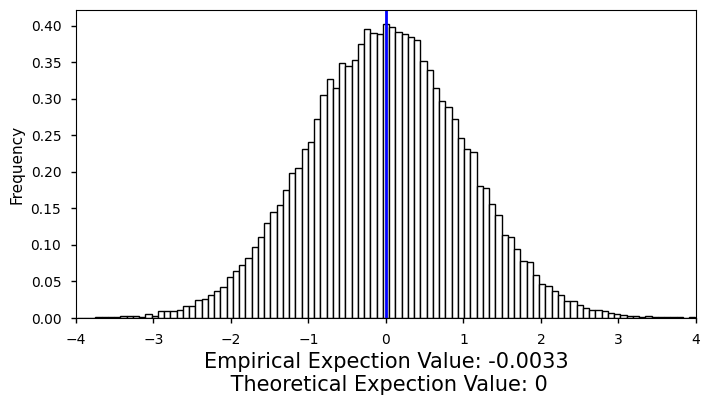
\includegraphics[width=0.6\textwidth]{images/nor_AR.png}
		\caption{Generating $N(0,1)$ with Accept - Reject method}
	\end{figure}

	If we want to generate normal random variable to have mean $\mu$  and variance $\sigma^2 $, just take $\mu +\sigma Z $.
\end{example}

\begin{example}[Generating Beta Distribution]
	\label{generate beta}
	If $\alpha$ and  $\beta $ are both getter then 1, then Beta density is uniformly bounded and its maximum attain at
	$\frac{\alpha-1}{\alpha+\beta-2}$. As a result the $U[0,1]$ density can be served as an envelope density for generating such Beta distribution by using accept-reject method.
	Precisely, generate $U$, $X\sim U[0,1]$ (independently), and retain the value if
	$U\le \frac{f(X)}{\sup_x f(X)}$, where,
	\[
		f(X)=\frac{\Gamma(\alpha+\beta)}{\Gamma(\alpha)\Gamma(\beta)}x^{\alpha-1} (1-x)^{\beta-1}, 0 < x< 1.
	\]
	Because
	\[
		\sup_x f(X) = f\left( \frac{\alpha-1}{\alpha+\beta-2} \right) = \frac{\Gamma(\alpha+\beta)}{\Gamma(\alpha)\Gamma(\beta)}\frac{(\alpha-1)^{\alpha-1} (\beta-1)^{\beta-1} }{(\alpha+\beta-2)^{\alpha+\beta-2} }
	\]
	The algorithm finally works out as follows:\\
	STEP 1: Generate independent $U,X \sim U[0,1]$.\\
	STEP 2: Retain the value $X$ if,
	\[
		U \le \frac{X^{\alpha-1} (1-X)^{\beta -1} (\alpha+\beta-2)^{\alpha+\beta-2} }{(\alpha-1)^{\alpha-1} (\beta-1)^{\beta-1} }.
	\]
	Otherwise, return to STEP 1.

	\begin{figure}[H]
		\centering
		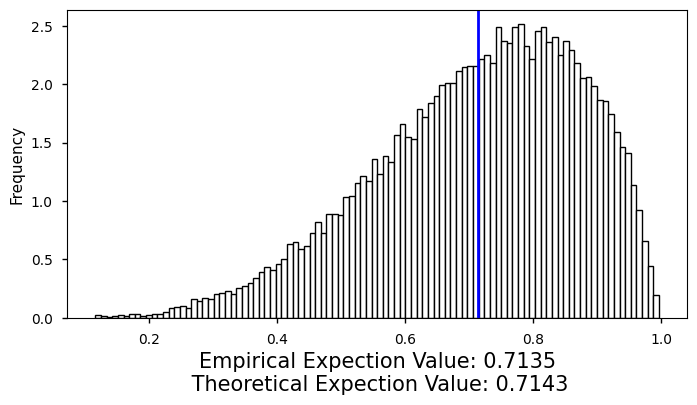
\includegraphics[width=0.6\textwidth]{images/beta_AR.png}
		\caption{Generating Beta(5,2) with accept-reject method}
		\label{Beta 5 2}
	\end{figure}
\end{example}

An issue about an accept-reject method is the acceptance rate.
Our goal make it as large as possible to increase the efficiency of the method.
This can be achieved by choosing $c$ to be smallest possible number, described in the result bellow.
\begin{theorem}[Acceptance Rate]
	For an accept-reject scheme, the probability that an $X\sim g$ is acceded is  $\frac{1}{c}$,
	and is maximized when $c$ is chosen to be $c=\sup_x\frac{f(x)}{g(x)}.$
\end{theorem}
\begin{proof}
	\begin{align*}
		P\left( U \le \frac{f(x)}{cg(x)} \right) & = \int_{-\infty}^{\infty} \int_{0}^{\frac{f(x)}{cg(x)}} g(t) du dt                                           \\
		                                         & = \int_{-\infty}^{\infty} \frac{f(t)}{cg(t)}g(t)dt = \int_{-\infty}^{\infty} \frac{f(t)}{c}dt = \frac{1}{c}.
	\end{align*}
	Because any $c$ that can be chosen must be at least as large as $\sup_x\frac{f(x)}{g(x)}$
	, obviously $1/c$ is maximized by choosing $c=\sup_x\frac{f(x)}{g(x)}.$
\end{proof}

In the example (\ref{generate normal}) for $N(0,1)$ the acceptance rate is $\sqrt{\frac{\pi}{2 e}} = 0.7601$.
And for example (\ref{generate beta}) for Beta(5,2) the acceptance rate is 0.4069

\subsection{Bivariate Techniques}
Let $X$ and $Y$ be independent slandered normal random variable and let $R$ and $\theta$
denote the polar coordinates of vector $(X,Y)$. That is,
\begin{align*}
	R^{2}       & = X^{2} + Y^2 \\
	\tan \theta & = \frac{Y}{X}
\end{align*}

Since $X$ and $Y$ are independent, their joint density is the product of their individual densities and thus given by
\begin{align*}
	f(x,y) & = \frac{1}{\sqrt{2\pi}} e^{-x^{2}/2 } \frac{1}{\sqrt{2\pi}} e^{-y^{2}/2 } \\
	       & = \frac{1}{2\pi} e^{-(x^{2}+y^{2})/2}
\end{align*}
To determine the joint density of $R^{2} $ and $\Theta$ - call it $g(d,\theta)$ we make the change of variables
\[
	d=x^{2}+y^{2}, \ \  \theta=\tan^{-1}\left( \frac{y}{x} \right)
\]
Then the joint density function of $d $ and $\Theta$ is,

\begin{align*}
    \label{jacobian transformation}
    g(d,\theta) &= |J| f(x,y) \\ 
                &= |J| \frac{1}{2\pi} e^{-(x^{2}+y^{2})/2} \numberthis
\end{align*}
where,
\[
	J =
	\begin{vmatrix}
        \frac{\partial x}{\partial t} & \frac{\partial x}{\partial \theta} \\[1ex]
		\frac{\partial y}{\partial t} & \frac{\partial y}{\partial \theta} \\
	\end{vmatrix} = \frac{1}{2}.
\]
Then, replacing the value of $ x = \sqrt{d}\sin(\theta)  $ and $ y=\sqrt{d}\cos(\theta) $ in the Equitation (\ref{jacobian transformation}) we get,
\begin{equation}
	g(d,\theta) = \frac{1}{2}\frac{1}{2\pi} e^{-d/2},\ \ \ 0< d<\infty, 0<\theta<2 \pi.
\end{equation}

As $g(d,\theta)$ is equal to product of the product of $Exp(1/2)$ density and $U(0,2 \pi)$, it follows that,\\
$R^{2}$ and $\Theta$ are independent, with $R^{2} \sim Exp(1/2)$ and $\Theta \sim U(0, 2 \pi)$ \\
Hence to generate a pair of independent slandered normal random variables $X$ and $Y$ by generating $R^{2} $ and $\Theta$ in polar coordinates and then
transform back to rectangular coordinates. Hence the algorithm is:\\
STEP 1: Generate random number $U_1, U_2 \sim U(0,1)$.\\
STEP 2: $ R^{2} = - 2 \ln U_1 $ and $\Theta = 2 \pi U_2 $. \\
STEP 3: Now let,
\begin{align*}
	X & = R \cos \Theta = \sqrt{-2\ln U_1}\cos(2 \pi U_2)                                   \\
	Y & = R \sin \Theta = \sqrt{-2 \ln U_1} \sin(2 \pi U_2). \label{Box-muller} \numberthis
\end{align*}

The transformation given by equitations (\ref{Box-muller}) are known as Box-Muller transformation.

\begin{figure}[H]
	\centering
	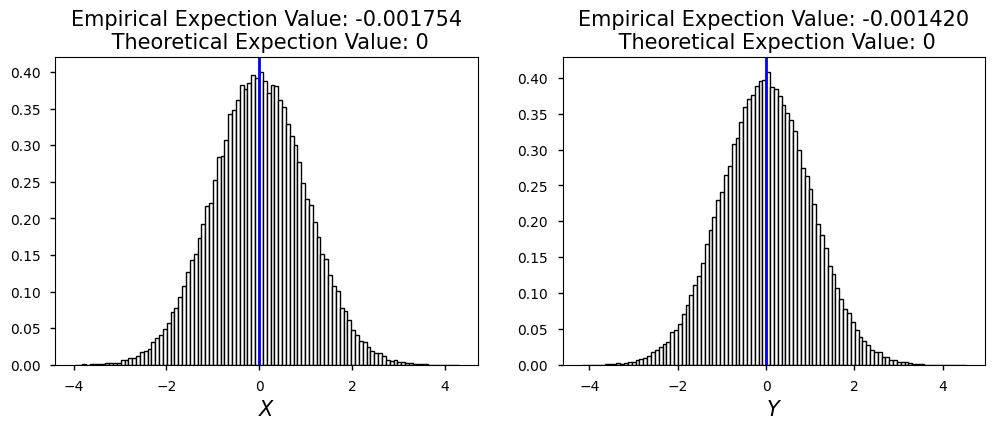
\includegraphics[width=0.9\textwidth]{images/nor_polar.png}
	\caption{Generating independent $X, Y \sim N(0,1)$ with polar method}
	\label{normal polar}
\end{figure}


\chapter{Ordinary Monte Carlo Simulation}
Polish-American mathematician Stanislaw Ulam, recovering from an illness, was playing a lot of
solitary card game. He wanted to calculate the probability of winning and
quickly it is impossible to calculate analytically. Then he thought about playing
lots of hands counting number of wins, but decided it will take years.
After falling several times he asked Von Neumann to build a program to simulate solitary
card game in ENIAC. Then Around 1940 they used Monte Carlo simulation in Manhattan Project
in which physicists wanted to understand how the physical
properties of neutrons would be affected by various possible scenarios following a
collision with a nucleus.

The basis for Monte Carlo is Law of Large Number. If we simulate large number $X_1, X_2, \ldots$ iid
copes of random variable $X$ Then we can approximate the true value $E(f(X))$ by simple mean
$\frac{1}{n}\sum_{i=1}^{n} f(X_i)$. Here in Monte Carlo Random Sampling play the key factor for good estimation of $E(f(X))$.

\section{Evaluate Integrals using Monte Carlo simulation}
The application of Monte Carlo is to computation of integrals. Let $g(x)$ be a function
and suppose we wanted to compute $I$ where
\[
	I = \int_{0}^{1} g(x) dx
\]

To compute the value of $I$, note that if $U\sim U[0,1]$ then we can express $I$ as
\[
	I = E[g(U)]
\]
If $U_1, \ldots, U_n$ are independent uniform $(0,1)$ random variables, it thus follows that
the random variables $g(U_1),\ldots,g(U_n)$ are independent and identically distributed random
variable having mean $I$. Therefore, by law of large numbers, its follows that,
with probability,
\[
	\sum_{i = 0}^{n} \frac{g(U_i)}{n} \to E(g(U))= I \text{ as } k \to \infty
\]

Hence we can approximate $I$ by generating a large number of random numbers $U_i$ and taking
as our approximation the average value of $g(U_i)$.

If we wanted to compute
\[
	I = \int_{a}^{b} g(x) dx
\]
then , by taking the substitute $y=(x-a)/(b-a)$, $dy = dx/(b-a)$, we see that
\begin{align*}
	I & = \int_{0}^{1} g(a+[b-a]y)(b-a)dy \\
	  & = \int_{ 0}^{1} h(y) dy
\end{align*}

Where $h(y)= (b-a)g(a+[b-a]y)$. Thus we can approximate $I$ by continually generating random
numbers and then taking the average value of $h$ evaluated at these random numbers.

Similarly, if we wanted
\[
	I = \int_{0}^{\infty} g(x) dx
\]

we could apply the substitution $y=1/(x+1)$, $dy=-dx/(x+1)^{2} = -y ^{2} dx$, to obtain the identity
\[
	I=\int_{0}^{1} h(y)dy
\]
where, \[
	h(y) = \frac{g(\frac{1}{y} -1)}{y ^{2}}
\]
Using this technique we can also evaluate multidimensional integrals. Suppose that $g$ is a function with n-dimention argument
and we are interested in computing
\[
	I = \int_{0}^{1} \int_{0}^{1} \ldots \int_{0}^{1} g(x_1, x_2 , \ldots , x_n) dx_1 dx_2 \ldots dx_2.
\]
Then, we can express $I$ as
\[
	I = E(g(U_1, U_2, \ldots U_n))
\]
where $U_1, U_2, \ldots U_n \sim U[0,1]$  Hence  if we generate $k$ independent sets, each consisting of $n$ independent $U[0,1]$
random variable
\begin{align*}
	U_1^{1}   & \ldots U_n^{1}  \\
	U_1^{2}   & \ldots U_n^{2}  \\
	          & \vdots          \\
	U_1^{k} , & \ldots, U_n^{k}
\end{align*}
then, since the random variables $g(U_1^{i},\ldots, U_n^{i}), i = 1,2,\ldots,k  $ are all independent and identically distributed
random variable with mean $I$, we can estimate $I$ by $\sum_{i = 1}^{k}g(U_1^{i} , \ldots, U_n^{i} )/k $.

\begin{example}
	Suppose we want to integrate,
	\[
		I = \int_{0}^{1} e^{-\frac{x ^{2}}{2}} dx.
	\]

	Then we can say that,
	\[
		I = E(e^{-\frac{U ^{2}}{2}})
	\]
	where, $U\sim U[0,1]$. Then simulating a large number of $U_1, U_2, \ldots, U_n\sim U[0,1]$ and calculating,
	\[
		\sum_{i = 1}^{n}  \frac{e^{-\frac{U_i ^{2}}{2}}}{n}
	\]
	we can evaluate $I$.

	Hence the algorithm is:\\
	STEP 1: Generate $U\sim U[0,1]$. \\
	STEP 2: Calculate $ e^{-\frac{U ^{2}}{2}} $ and retain it. goto STEP 1. \\
	STEP 3: After large number of iteration evaluate the average.
	\begin{table}[H]
		\begin{center}
			\begin{tabular}{l c}
				\hline
				Monte Carlo sample size & Monte Carlo Estimate of I = 0.8556 \\
				\hline
				50                      & 0.8555                              \\
				100                     & 0.8558                              \\
				1000                    & 0.8555                              \\
				10000                   & 0.8556                              \\
				100000                  & 0.8556                              \\
				\hline
			\end{tabular}
			\caption{Monte Carlo Integration of $e^{-x ^{2}/2}$.}
		\end{center}
	\end{table}
	\begin{figure}[H]
		\centering
		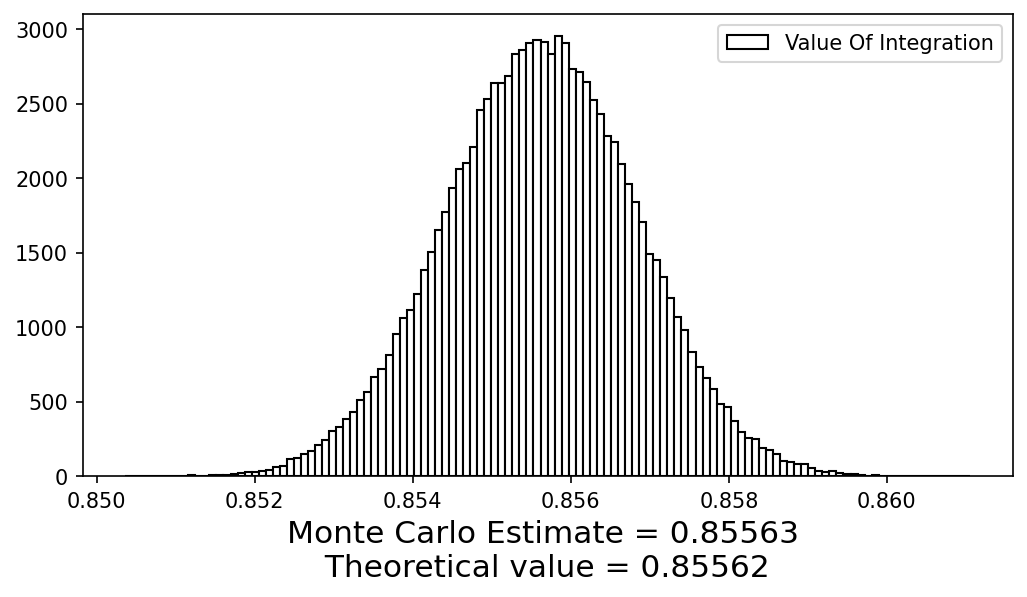
\includegraphics[width=0.6\textwidth]{images/evaluating_integration.png}
		\caption{Monte Carlo Integration of $e^{-x ^{2}/2} $}
	\end{figure}
	Here, we see by the time the Monte Carlo sample size is 100000, we get fairly
	accurate estimates for the value $I$.
\end{example}

\section{The Estimation of $\pi$}
Suppose that the random vector $(X,Y)$ is uniformly distribution in the square of area 4
centered at the origin. That is, it is a random point in the region specified in Figure \ref{Square}.
Let us consider now the probability that this random point in the square in contained within the inscribed circle of radius 1
like the Figure \ref{Circle within Square}.

\begin{figure}[H]
	\centering
	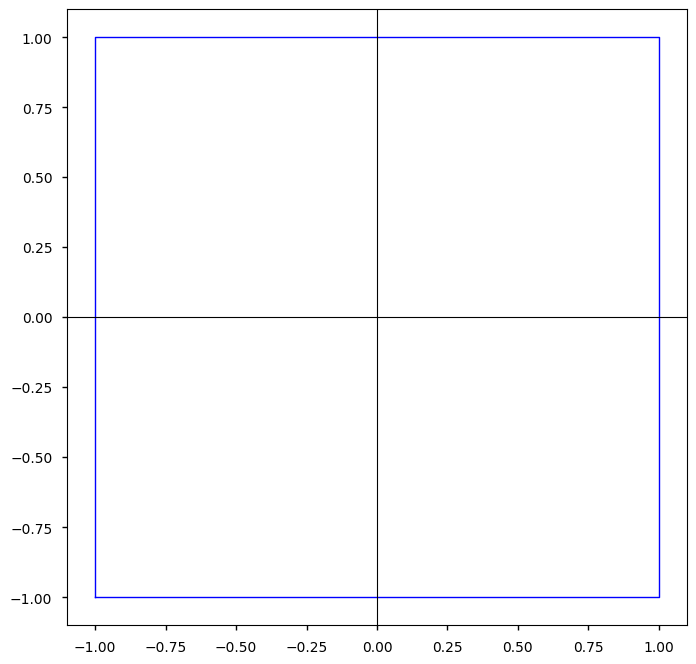
\includegraphics[width=0.4\textwidth]{images/square.png}
	\caption{Square}
	\label{Square}
\end{figure}

\begin{figure}[H]
	\centering
	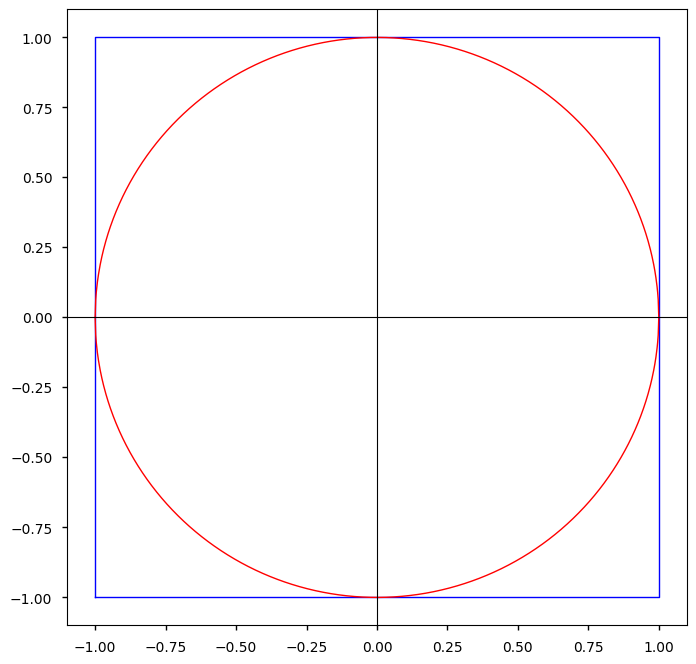
\includegraphics[width=0.4\textwidth]{images/circle.png}
	\caption{Circle within Square}
	\label{Circle within Square}
\end{figure}

Note that since $(X,Y)$ is uniformly distributed in the square it follows that
\begin{align*}
	P((X,Y) \text{ is in the circle } ) & = P(X ^{2}+ Y ^{2}\le 1)                                                        \\
	                                    & = \frac{\text{Area of the circle} }{\text{Area of the square} } = \frac{\pi}{4}
\end{align*}

Hence we generate a large number of points in the square, the proportion of points that fall within the circle will be approximately $\pi/4$.
Now, if $X$ and $Y$ were independent and both were uniformly distributed over $(-1,1)$, their joint density would be
\begin{align*}
	f(x,y) & = f(x)f(y)                                         \\
	       & = \frac{1}{2} \times \frac{1}{2}                   \\
	       & = \frac{1}{4} , \  -1 \le x \le 1,\ -1 \le y \le 1
\end{align*}

Since, the density function of $(X,Y)$ is constant in the square, it thus follows that $(X,Y)$ is uniformly distributed in the square.
Now, if $U\sim U[0,1]$ then $2U\sim U[0,2]$ and so $2U-1\sim U[-1,1]$. Therefore, if we generate ranom numbers $U_1 \text{ and }  U_2$
and set $X=2U_1 - 1$ and $Y= 2U_2-1$, and define,
\[
	I = \begin{cases}
		1 \text{ if } X ^{2} + y ^{2} \le 1 \\
		0 \text{ otherwise }
	\end{cases}
\]
Then,
\[
	E(I)=P(X ^{2} + y ^{2} \le 1) = \frac{\pi}{4}.
\]
Hence the Algorithm for estimating $\pi$ is:\\
STEP 1: Set Circle = 1. \\
STEP 2: Generate $U_1, U_2\sim U[0,1]$\\
STEP 3: If $(2U_1-1)^{2}+ (2U_2-1)^{2} \le 1$ Set Circle = Circle + 1, Otherwise return to STEP 2.
STEP 4: After simulating $N$ time, set $\text{Area of Circle}  = \text{Circle}  / N$

\begin{table}[H]
	\centering
	\begin{tabular}{l c}
		\hline
		Monte Carlo sample & Monte Carlo Estimate of $\pi$ \\
		\hline
		50                 & 2.9600                        \\
		100                & 3.0800                        \\
		1000               & 3.1200                        \\
		10000              & 3.1428                        \\
		100000             & 3.1397                        \\
		1000000            & 3.1394                        \\
		10000000           & 3.1414                        \\
		\hline
	\end{tabular}
	\caption{Monte Carlo Estimates of $\pi$}
	\label{tab:montecarlopi}
\end{table}
Here, we see by the time the Monte Carlo sample size is 10000000, we get fairly accurate estimates for $\pi$



\section{Importance Sampling}
There are two different ways to think about importance sampling.
The more traditional one is to go back to the primary problem that
Monte Carlo  wants to solve,
namely to approximate the value of an expectation
$\mu = \int \phi_0(x)dF_0(x) $ for some function $\phi_0$ and some CDF $F_0$.
However, $(\phi_0,F_0)$ is not the only pair $(\phi,F)$ for which
$\int \phi(x)dF(x) $ equals the specific number $\mu$. Indeed, given any other
CDF $F_1$,
\begin{align*}
	\mu & = \int \phi_0(x)dF_0(x)                      \\
	    & = \int \phi_0(x)\frac{dF_0}{dF_1}(x) dF_1(x) \\
	    & = \int \lambda(x)\phi_0(x)dF_1(x).
\end{align*}

where $\lambda(x)=\frac{dF_0}{dF_1}(x)$. If $F_0$, $F_1$ have densities
$f_0$, $f_1$, then $\lambda(x)=\frac{f_0(x)}{f_1(x)}$; if $F_0,$ $F_1$
have respective pmfs $f_0$, $f_1$, then also $\lambda(x)=\frac{f_0(x)}{f_1(x)}$
This raises the interesting possibility that we can sample from a general $F_1$, and
subsequently use the usual Monte Carlo estimate
\[
	\hat{\mu} = \frac{1}{n} \sum_{i = 1}^{n} \lambda(X_i)\phi_0(X_i) = E_{F_1}[\lambda(X_i)\phi_0(X_i)].
\]

where $X_1, X_2, \ldots, X_n$ is Monte Carlo sample from $F_1$.
Importance sampling poses the problem of finding an optimal choice of $F_1$ for which to sample,
so that $\hat{\mu}$ has the smallest possible variance.
The distribution $F_1$ hat ultimately gets
chosen is called the \textit{importance sampling distribution}.

We can visualize this method by an example.

\begin{example}
	\label{ex:reductionofvariance}
	Suppose we want to evaluate
	\[
		I = \int_{0}^{10} e^{-2 |x-5|} dx.
	\]
	doing it analytically we get $I = 0.9999$.

	Now, suppose $\phi(x) = e^{-2 |x-5|}$ then we want to evaluate
	\[
		I = \int_{0}^{10} \phi(x) dx
	\]
	Now,
	\begin{align*}
		\label{hx with U}
		I & = \int_{0}^{10} \phi(x) dx                                                                                                            \\
		  & = \int_{0}^{10} \phi(x)\frac{10}{10} dx                                                                                               \\
		  & = \int_{0}^{10} 10 \times \phi(x) \frac{1}{10} dx = \int_{0}^{10} 10\phi(x) f_0(x) dx \text{ where } f_0(x)\text{ pdf of }U(0,1) \numberthis \\
		  & = E_U[10 \times \phi(U)] \text{ where, }  U\sim U(0,10).
	\end{align*}

	By Ordinary Monte Carlo technique we can estimate $I$ by $\frac{1}{N}\sum_{i = 1}^{N} 10 \times \phi(U_i)$ where $U_i\sim U(0,10)$ for $i=1,2,\ldots,N$
	for the large number of $N$.
	\begin{figure}[H]
		\centering
		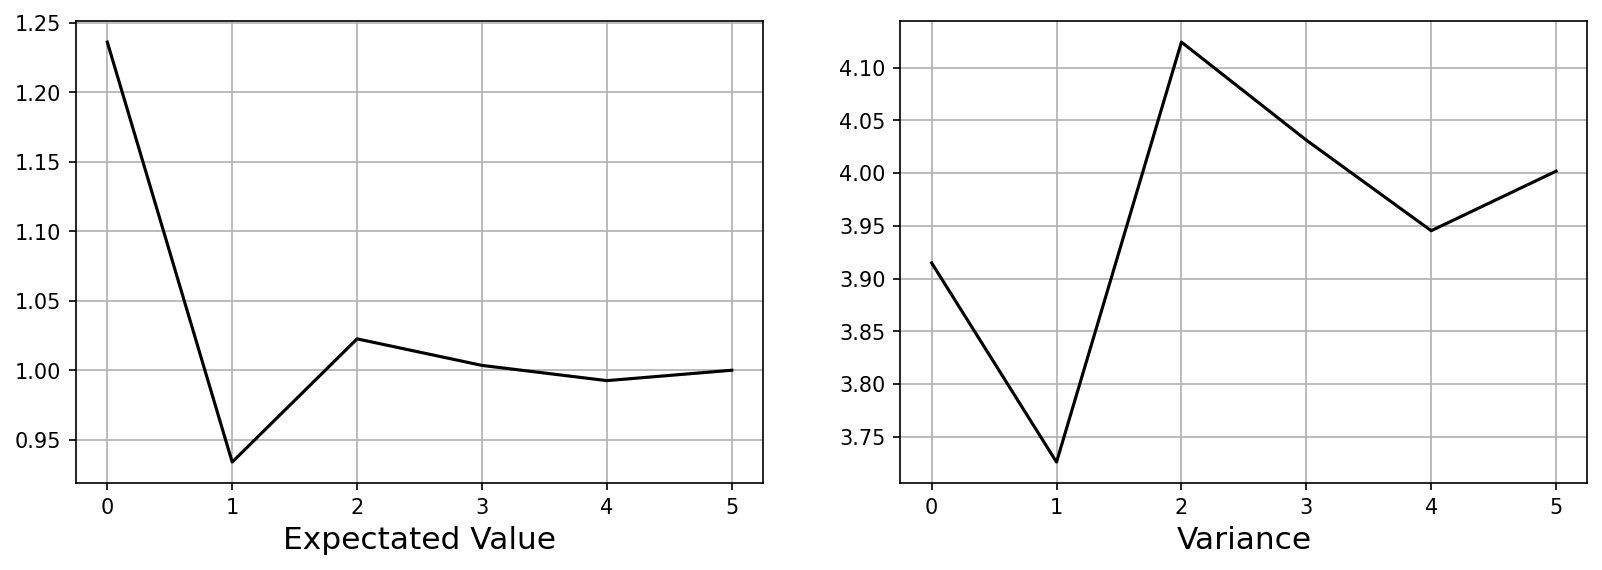
\includegraphics[width=0.8\textwidth]{int_h(x)_MC.png}
		\caption{Monte Carlo integration of $\int_{0}^{10} e^{-2 |x-5|} dx$.}
		\label{MC:IntegrationOFe-2|x*5|}
	\end{figure}
	\begin{table}[h]
		\centering
		\begin{tabular}{lcc}
			\hline
			Sample Size & Estimated Value I=0.9999 & Variance \\
			\hline
			10          & 2.3243                   & 5.6912   \\
			100         & 1.0372                   & 3.6717   \\
			1000        & 0.8871                   & 3.5543   \\
			10000       & 1.0467                   & 4.2416   \\
			100000      & 1.0053                   & 4.0089   \\
			1000000     & 1.0054                   & 4.0346   \\
			\hline
		\end{tabular}
		\caption{Monte Carlo integration of $\int_{0}^{10} e^{-2 |x-5|} dx$.}
		\label{tab:IntegrationOFe-2|x*5|}
	\end{table}
	Here we can see that for sample size 1M, we get a pretty good estimation of $I$ with less then $0.6\%$ error. But the variance is very high.
	If we see at left of \Cref{fig:hxwithU01andN01} we can see we are taking unnecessary value from low frequency part of $\phi(x)$ that is,
	from extreme left and right. If we choose an importance sampling distribution that has similar curve as $\phi(x)$, then we can estimate $I$ with low variance.
	If we choose importance sampling distribution as $N(5,1)$ then we see from right of \Cref{fig:hxwithU01andN01} it has similar pattern as $\phi(x)$.
	\begin{figure}[H]
		\centering
		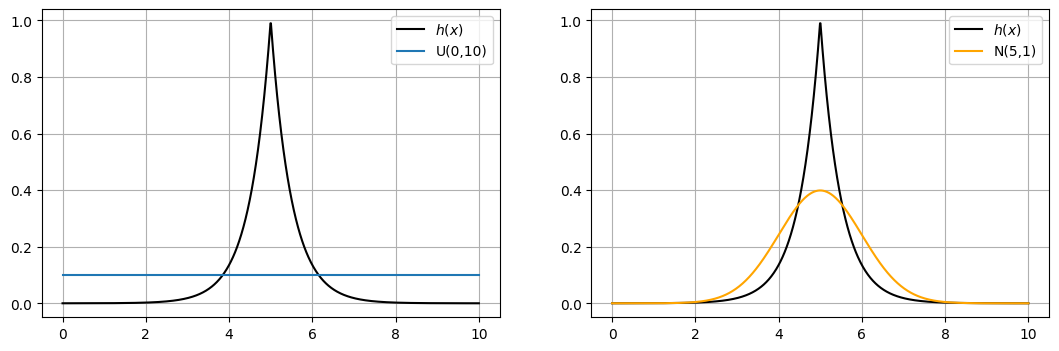
\includegraphics[width=0.8\textwidth]{h(x)_with_normal_and_uniform.png}
		\caption{$h(x)$ with $U(0,10)$ and $N(5,1)$}
		\label{fig:hxwithU01andN01}
	\end{figure}

	Let, $f_1(x)$ is pdf of $N(0,1)$ then, from \Cref{hx with U}
	\begin{align*}
		I & = \int_{0}^{10} 10\phi(x) f_0(x) dx                                            \\
		  & = \int_{0}^{10} 10 \phi(x) \frac{f_0(x)}{f_1(x)} q(x)dx                          \\
		  & = E_X\left[ 10 \phi(X) \frac{f_0(X)}{f_1(X)} \right] \text{ where } X\sim N(5,1) \\
		  & = E_X\left[ 10 \phi(X) \lambda(X) \right]\text{ where } X\sim N(5,1)
	\end{align*}
	Where, $\lambda(x) = \frac{f_0(x)}{f_1(x)}$ here $f_0(x)$ is pdf of $U(0,1)$ and $f_1(x)$ is pdf of $N(5,1)$. Now using usual Monte Carlo estimate
	\[
		I = \frac{1}{N} \sum_{i = 1}^{N} 10 \phi(X_i) \lambda(X_i)
	\]
	where $X_1, X_2,\ldots,X_N$ is Monte Carlo sample from $N(5,1)$.
	\begin{table}[H]
		\centering
		\begin{tabular}{l c c}
			\hline
			Sample Size & Estimated Value (I=0.9999) & Variance \\
			\hline
			10          & 1.2473                     & 0.3812   \\
			100         & 0.9292                     & 0.2593   \\
			1000        & 1.0018                     & 0.3550   \\
			10000       & 1.0072                     & 0.3603   \\
			100000      & 1.0039                     & 0.3595   \\
			1000000     & 0.9999                     & 0.3580   \\
			\hline
		\end{tabular}
		\caption{Evaluating $\int_{0}^{10} e^{-2 |x-5|} dx$ using Importance Sampling.}
		\label{tab:mytable}
	\end{table}
	
	\begin{figure}[H]
		\centering
		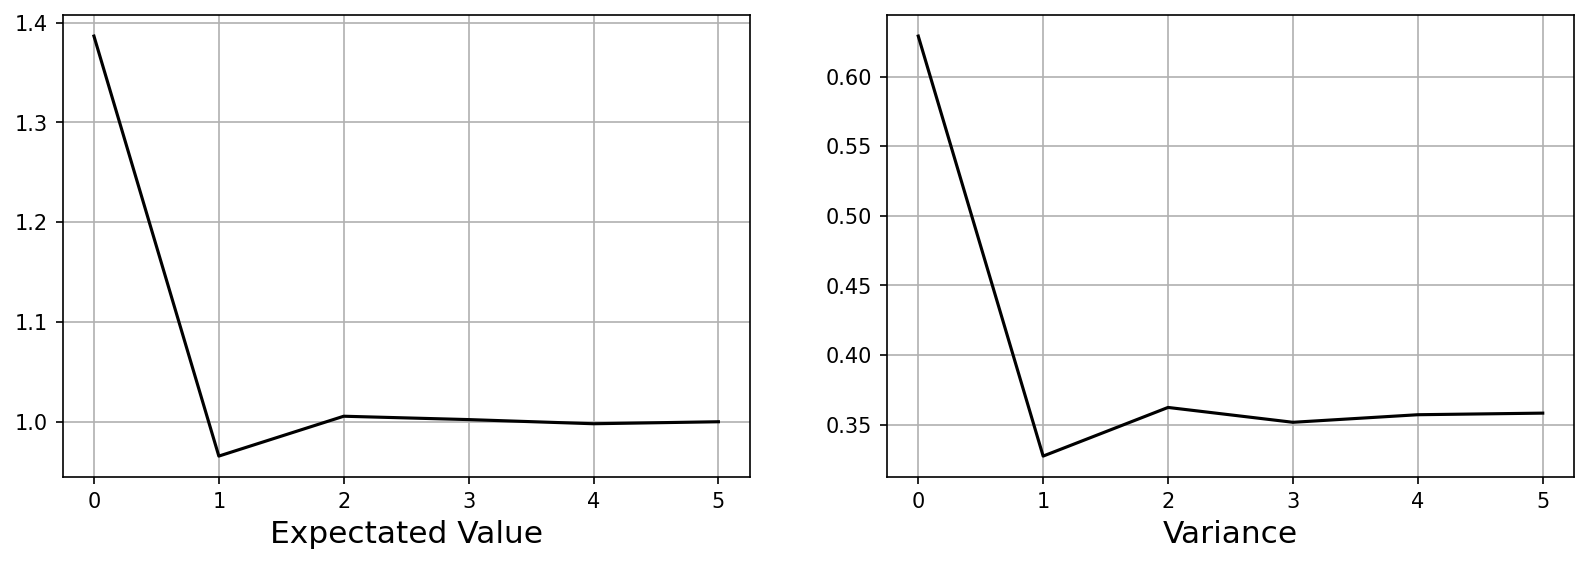
\includegraphics[width=0.8\textwidth]{int_h(x)_ipsam.png}
		\caption{Evaluating $\int_{0}^{10} e^{-2 |x-5|} dx$ using Importance Sampling.}
		\label{fig:impotrancesampling1}
	\end{figure}
	Here we can see that the estimation of $I$ is pretty close and variance is also
	lower the Original Monte Carlo method.
\end{example}

A more contemporary view of importance sampling is that we do not approach
importance sampling as an optimization problem, but because the circumstances
force us to consider different sampling distributions $F$.

Now, we also assume that $F_0,$ $F_1$ both have densities, say $f_0$, $f_1$.
If $F_0$, $F_1$ are both discrete then the notation only change but the argument is same.
Suppose then $f_i(x)=\frac{h_i(x)}{c_i},\ i=0,1$, where the assumption is that $h_0$, $h_1$
are completely known and also computable, but $c_0$, $c_1$ are unknown and are not even computable.
Then, as we showed above, for any function $\phi$ for which the expectation $E_{F_0}[\phi(X)]$ exist,

\begin{align*}
	\mu & = E_{F_0}[\phi(X)] := \int \frac{f_0(x)}{f_1(x)}\phi(x)f_1(x)dx      \\
	    & =\frac{c_1}{c_0} \int \frac{\phi(x)h_0(x)}{h_1(x)}f_1(x)dx           \\
	    & =\frac{c_1}{c_0} E_{F_1}\left( \frac{\phi(X)h_0(X)}{h_1(X)} \right).
\end{align*}

This is a useful reduction, but we have to deal with the fact that ratio $\frac{c_1}{c_0}$
is not known to us. Now, if we use the special function $\phi(x)\equiv 1$, the same
representation above gives us
\begin{align*}
	1                        & = \frac{c_1}{c_0} E_{F_1} \left( \frac{h_0(X)}{h_1(X)} \right) \\
	\implies \frac{c_1}{c_0} & = \frac{1}{E_{F_1} \left( \frac{h_0(X)}{h_1(X)} \right)}
\end{align*}
and because $h_0,$ $h_1$ are explicitly known to us, we have a way to get rid of the
quotient $\frac{c_1}{c_0}$ and write the final \textit{importance sampling identity}
\begin{align*}
	E_{F_0}[\phi(x)] = \frac{E_{F_1}\left( \frac{\phi(X)h_0(X)}{h_1(X)} \right)}{E_{F_1} \left( \frac{h_0(X)}{h_1(X)} \right)}
\end{align*}
We can now use an available Monte Carlo sample $X_1,X_2,\ldots,X_n$ from $F_1$
to find Monte Carlo estimates for $\mu = E_{F_0}[\phi(x)]$

The basic plug-in estimate for $\mu$ is the so-called ratio estimate
\[
	\hat{\mu} = \frac{\sum_{i = 1}^{n}\frac{\phi(X_i)h_0(X_i)}{h_1(X_i)} }{\sum_{i = 1}^{n} \frac{h_0(X_i)}{h_1(X_i)}}.
\]

\begin{example}[Binomial Bayes problem with an Atypical Prior]
	\label{Binomial Bayes problem with an Atypical Prior}
	Suppose $X\sim Bin(m,p)$ for some fixed $m$ and $p$ has the prior density $c\sin^{2}(\pi p)$,
	where $c$ is a normalizing constant.
	Throughout the example, $c$ denotes a generic constant,
	and is not intended to mean the same constant at every use.

	The posterior density of $p$ given $X = x$ is
	\[
		\pi(p|X=x) = cp^{x}(1-p)^{m-x}\sin ^{2}(\pi p), \ \ 0<p<1.
	\]
	The problem is to find the posterior mean
	\[
		\mu = c \int_{0}^{1} p[cp^{x}(1-p)^{m-x}\sin ^{2}(\pi p)]dp.
	\]

	We use importance sampling to approximate the value of $\mu$. Towards this, choose
	\[
		\phi(p)=p, \ h_0(p) = p^{x} (1-p)^{m-x} \sin ^{2}(\pi p),\ h_1(p) = p^{x}(1-p)^{m-x},
	\]
	so that if $p_1,p_2,\ldots,p_n$ are samples from $F_1$, (i.e. $p_i\sim Beta(x+1, m-x+1)$),
	then the importance sampling estimate of the posterior mean $\mu$ is
	\begin{align*}
		\hat{\mu} & = \frac{\sum_{i=1}^{n}\frac{\phi(p_i)h_0(p_i)}{h_1(p_i)} }{\sum_{i=1}^{n}\frac{h_0(p_i)}{h_1(p_i)} } \\
		          & = \frac{\sum_{i=1}^{n}p_i\sin ^{2}(\pi p_i) }{\sum_{i=1}^{n} \sin ^{2}(\pi p_i) }.
	\end{align*}

	Note that we did not need to calculate the normalizing constant in the posterior density.
	We take $m=100$, $x=45$ for specificity.
	\begin{table}[H]
		\centering
		\begin{tabular}{l p{4.5cm} p{2cm}}
			\hline
			Sample Size & Importance Sampling Estimate of $\mu$ & Variance \\
			\hline
			20          & 0.4821                                & 0.5465   \\
			50          & 0.4629                                & 0.5162   \\
			100         & 0.4597                                & 0.4929   \\
			250         & 0.4635                                & 0.4902   \\
			500         & 0.4585                                & 0.4962   \\
			\hline
		\end{tabular}
		\caption{Importance Sampling Estimates of $\mu$ for Different Sample Sizes}
		\label{tab:importance-sampling-mu}
	\end{table}
    \begin{figure}[H]
        \centering
        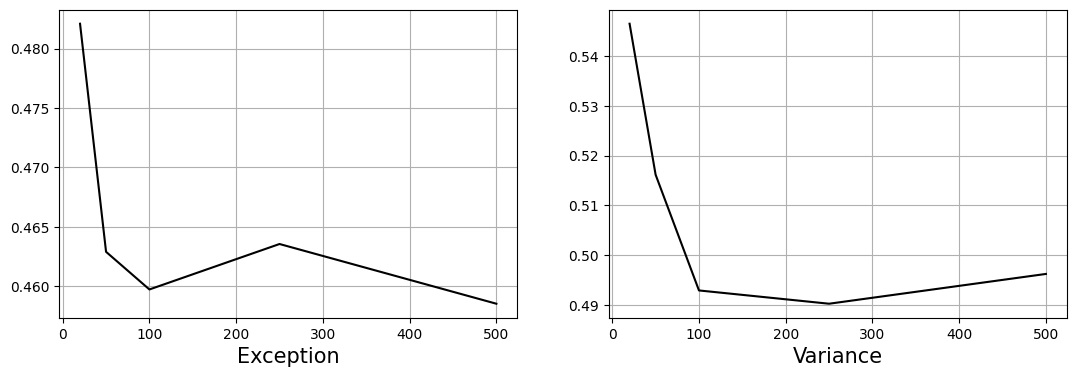
\includegraphics[width=0.8\textwidth]{chap4ex2.png}
        \caption{Exception and variance graph of Binomial Bayes problem with an Atypical Prior}
    \end{figure}
\end{example}

\subsection{Optimal Importance Sampling Distribution}
We now address the question of the optimal choice of the importance sampling
distribution. There is no unique way to define what an optimal choice means. We
formulate one definition of optimality and provide an optimal importance sampling
distribution. The optimal choice would not be practically usable, as we shown.
However, the solution still gives useful insight.

\begin{theorem}
	Consider the importance sampling estimator $\hat{\mu} = \frac{1}{n}\sum_{i=1}^{n} \lambda(X_i)\phi(X_i) $ for $\mu=\int \phi(x)f_0(x)dx $, where
	$\lambda(x) =\frac{f_0(x)}{f_1(x)}$, and $X_1,\ldots,X_n$ are iid observations from $F_1$
	Assume that $\phi(x)\ge0$, and $\mu>0$. Then, $Var_{F_1}(\hat{\mu})$ is
	minimized when $f_1(x)=\frac{\phi(x)f_0(x)}{\mu}$.
\end{theorem}
\begin{proof}
	Because $X_1,\ldots,X_n$ is iid, so are $\lambda(X_1)\phi(X_1),\ldots,\lambda(X_n)\phi(X_n)$, and hence,
	\[
		Var_{F_1}(\hat{\mu}) = \frac{1}{n} Var_{F_1}(\lambda(X_1)\phi(X_1))
		.
	\]

	Clearly, this is minimized when with probability one under $F_1$, $\lambda(X_1)\phi(X_1)$
	is constant, say $k$. The constant $k$ must be equal to the mean of $\lambda(X_1)\phi(X_1)$, that is,
	\begin{align*}
		k & = \int \lambda(x)\phi(x)f_1(x)dx              \\
		  & = \int \frac{\phi(x)f_0(x)}{f_1(x)} f_1(x) dx \\
		  & = \int \phi(x)f_0(x)dx = \mu.
	\end{align*}
	Therefore, the optimal importance sampling density satisfies $\lambda(x)\phi(x) = \mu$
	hence,
	\[
		f_1(x) = \frac{\phi(x)f_0(x)}{\mu}.
	\]
\end{proof}
This is not usable in practice, because it involves $\mu$,which is precisely the unknown number we want to approximate.
However, the theoretically optimal solution
suggests that the importance sampling density should follow key properties of the
unnormalized function $\phi(x)f_0(x)$.
For example, $f_1$ should have the same shape and tail behavior as $\phi(x)f_0(x)$.

We have seen this phenomena in the \Cref{Binomial Bayes problem with an Atypical Prior}.
Because Graph of $\phi(x)h_0(x)$ and $h_1(x)$ in \Cref{fig:ch4ex2plothx}, they both have the same key properties.   
\begin{figure}[H]
    \centering
    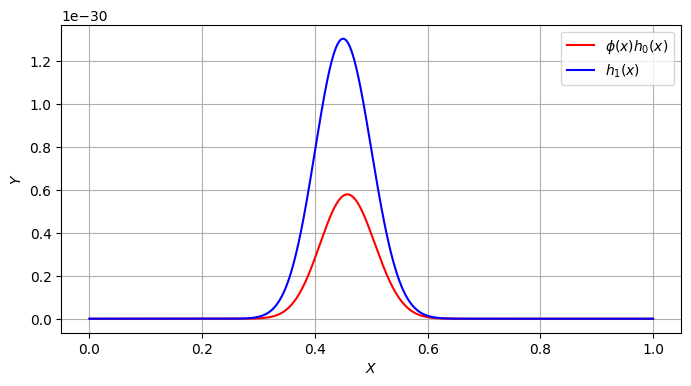
\includegraphics[width=0.6\textwidth]{ch4ex2plot_hx.png}
    \caption{Graph of $\phi(x)h_0(x)$ and $h_1(x)$}
    \label{fig:ch4ex2plothx}
\end{figure}


\nocite{*}
\bibliographystyle{plain}
\bibliography{Referance}

\end{document}
